% !TEX root =  ../supplementary.tex
\section{A Bivariate Joint Model for the Longitudinal PSA, and DRE Measurements, and Time to Cancer Progression}
\label{sec:jm_framework}
In this appendix section, we first provide a short introduction to the world's largest active surveillance (AS) program called Prostate Cancer Research International Active Surveillance, abbreviated as PRIAS \citep{bul2013active}, that we use to develop our methodology. We then present an introduction to the joint models for time-to-event and longitudinal data \citep{tsiatis2004joint,rizopoulos2012joint}, that we fit to the PRIAS dataset.  Lastly, we present the parameter estimation for our model using the Bayesian approach. 

\subsection{PRIAS Dataset}
The PRIAS dataset consists of 5270 AS patients, of which 866 observe cancer progression. For each patient, prostate-specific antigen (PSA) measurements (ng/mL) are scheduled every 3 months for first 2 years and every 6 months thereafter. The DRE measurements are scheduled every 6 months. We use the DRE measurements after converting them on a binary scale, namely $\mbox{DRE} > \mbox{T1c}$ and $\mbox{DRE} \leq \mbox{T1c}$ \cite{schroder1992tnm}. On average 5 DRE and 9 PSA measurements have been recorded per patient. Larger values for PSA and/or larger score for DRE, may indicate cancer progression. However, it is the occurrence of biopsy Gleason score larger than 6, that is commonly considered cancer progression. In PRIAS study, biopsies are scheduled at the  following fixed follow-up times (measured since inclusion in AS): year 1, 4, 7, and 10, and every 5 years thereafter. An annual schedule of biopsies is prescribed to those patients who have a PSA doubling time between 0 and 10 years. The PSA doubling time at any point during follow-up is measured as the inverse of the slope of the regression line through the base two logarithm of the observed PSA values.

\subsection{Model Definition}
\label{subsec:model_def}
Let $T_i^*$ denote the true cancer progression time for the $i$-th patient in PRIAS. Since biopsies are conducted periodically, $T_i^*$ cannot be observed directly and it is only known to fall in an interval ${l_i < T_i^* \leq r_i}$, where $r_i$ and $l_i$ are the time of the latest and second latest biopsies, respectively, if the progression is observed at the latest biopsy. When the progression is not observed, then $l_i$ is the time of the latest biopsy and $r_i = \infty$. Further, let $\boldsymbol{y}_{di}$, and $\boldsymbol{y}_{pi}$ denote the $n_{di} \times 1$, and $n_{pi} \times 1$ vectors of the DRE, and PSA longitudinal measurements, respectively. For a sample of $n$ patients the observed data is denoted by ${\mathcal{D}_n = \{l_i, r_i, \boldsymbol{y}_{di}, \boldsymbol{y}_{pi}; i = 1, \ldots, n\}}$.

The patient-specific PSA and DRE measurements over time are modeled using a generalized linear mixed effects model. For the $i$-th patient, the mixed effects sub-model for DRE is given by:
\begin{equation}
\label{eq:long_model_dre}
\begin{split}
    \mbox{logit} \big[\mbox{Pr}\{y_{di}(t) > \mbox{T1c}\}\big] &= \beta_{0d} + b_{0di} + (\beta_{1d} + b_{1di}) t\\
    &+ \beta_{2d} (\mbox{Age}_i-70) + \beta_{3d} (\mbox{Age}_i-70)^2
    \end{split}
\end{equation}
where, $t$ denotes a specific time point in the AS follow-up, $\mbox{Age}_i$ is the age of the $i$-th patient at the time of inclusion in AS. The fixed effect parameters are denoted by $\{\beta_{0d}, \ldots, \beta_{3d}\}$, and $b_{0di}, b_{1di}$ are the patient specific random effects. With this definition, we assume that the log odds of obtaining a DRE score larger than T1c remain linear over time. An example model fit for DRE is shown in panel A of Figure~\ref{fig:jmExplanationPlot_1757}. For the $i$-th patient, the mixed effects sub-model for PSA is given by:
\begin{equation}
\label{eq:long_model_psa}
\begin{split}
    \log_2 \big\{y_{pi}(t) + 1\big\} &= m_{pi}(t) + \varepsilon_{pi}(t),\\
    m_{pi}(t) &= \beta_{0p} + b_{0pi} + \sum_{k=1}^4 (\beta_{kp} + b_{kpi})  B_k(t,\mathcal{K})\\ 
    &+ \beta_{5p} (\mbox{Age}_i-70) + \beta_{6p} (\mbox{Age}_i-70)^2,
    \end{split}
\end{equation}
where, $m_{pi}(t)$ denotes the underlying measurement error free value of $\log_2 (\mbox{PSA} + 1)$ transformed \citep{pearson1994mixed,lin2000latent} measurements at time $t$. To accommodate for a non-linear evolution of this value over the follow-up period in AS, we utilize B-splines \citep{de1978practical}. In Equation (\ref{eq:long_model_psa}), $B_k(t, \mathcal{K})$ denotes the $k$-th basis function of a B-spline with three internal knots at $\mathcal{K} = \{0.1, 0.7, 4\}$ years, and boundary knots at 0 and 5.42 years (0.95 quantile of the observed follow-up times). The fixed effect parameters are denoted by $\{\beta_{0p},\ldots,\beta_{6p}\}$ and the patient specific random effects are denoted by $\{b_{0pi}, \ldots, b_{4pi}\}$. The error $\varepsilon_{pi}(t)$ is assumed to be t-distributed with three degrees of freedom (see Appendix~B.1) and scale $\sigma$, and is independent of the random effects. An example model fit for PSA is shown in panel B of Figure~\ref{fig:jmExplanationPlot_1757}. To account for the association between the DRE and PSA measurements, we link their corresponding random effects. More specifically, the complete vector of random effects ${\boldsymbol{b}_i = (b_{0di}, b_{0di}, b_{0pi}, \ldots, b_{4pi})^T}$ is assumed to follow a multivariate normal distribution with mean zero and ${7\times 7}$ variance-covariance matrix $\boldsymbol{D}$.
\begin{figure}[!htb]
\captionsetup{justification=justified}
\centerline{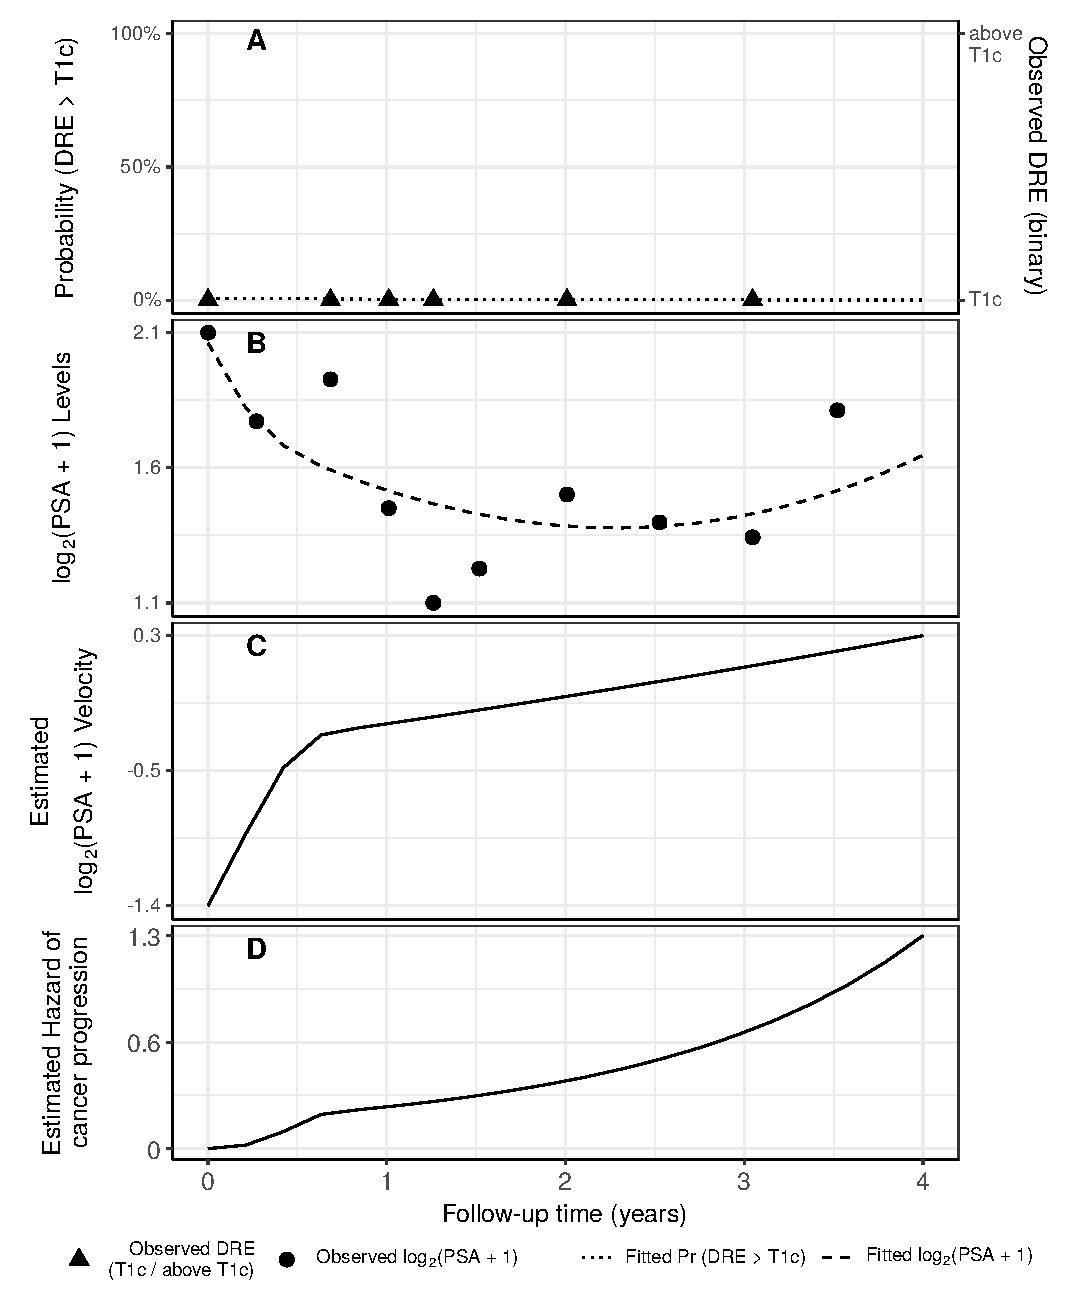
\includegraphics[width=\columnwidth]{images/jmExplanationPlot_1757.eps}}
\caption{Illustration of the joint model fitted to the PRIAS dataset. \textbf{Panel~A:} shows the observed DRE scores and the fitted probability of obtaining a DRE score greater than T1c (Equation~\ref{eq:long_model_dre}). \textbf{Panel~B:} shows the observed and fitted $\log_2(\mbox{PSA} + 1)$ levels (Equation~\ref{eq:long_model_psa}). \textbf{Panel~C:} shows the estimated $\log_2(\mbox{PSA} + 1)$ velocity (velocity cannot be observed directly) over time. The hazard function (Equation~\ref{eq:rel_risk_model}) shown in \textbf{Panel~D}, depends on the fitted log odds of having a $\mbox{DRE} > \mbox{T1c}$, and the fitted $\log_2(\mbox{PSA} + 1)$ value and velocity.}
\label{fig:jmExplanationPlot_1757}
\end{figure}

To model the impact of DRE and PSA measurements on the risk of cancer progression, we use a relative risk sub-model. More specifically, the hazard of cancer progression $h_i(t)$ at a time $t$ is given by:
\begin{equation}
\label{eq:rel_risk_model}
\begin{split}
    h_i(t) &= h_0(t) \exp\Big(\gamma_1 (\mbox{Age}_i-70) + \gamma_2 (\mbox{Age}_i-70)^2\\
    &+\alpha_{1d} \times \mbox{logit} \big[\mbox{Pr}\{y_{di}(t) > \mbox{T1c}\}\big]+ \alpha_{1p} \times m_{pi}(t) + \alpha_{2p} \times \frac{\partial m_{pi}(t)}{\partial {t}}\Big),
    \end{split}
\end{equation}
where, $\gamma_1, \gamma_2$ are the coefficients for the effect of age. The parameter $\alpha_{1d}$ models the impact of log odds of obtaining $\mbox{DRE} > \mbox{T1c}$ on the hazard of cancer progression. The impact of PSA on the hazard of cancer progression is modeled in two ways, namely at any time $t$ the effect of the instantaneous underlying value (dashed line in panel B of Figure~\ref{fig:jmExplanationPlot_1757}) of PSA $m_{pi}(t)$ is given by $\alpha_{1p}$, and the effect of the instantaneous underlying PSA velocity $\partial m_{pi}(t)/\partial {t}$ (panel C in Figure~\ref{fig:jmExplanationPlot_1757}) is given by $\alpha_{2p}$. Lastly, $h_0(t)$ is the baseline hazard at time t, and is modeled flexibly using P-splines \citep{eilers1996flexible}. More specifically:
\begin{equation*}
\log{h_0(t)} = \gamma_{h_0,0} + \sum_{q=1}^Q \gamma_{h_0,q} B_q(t, \boldsymbol{v}),
\end{equation*}
where $B_q(t, \boldsymbol{v})$ denotes the $q$-th basis function of a B-spline with knots $\boldsymbol{v} = v_1, \ldots, v_Q$ and vector of spline coefficients $\gamma_{h_0}$. To avoid choosing the number and position of knots in the spline, a relatively high number of knots (e.g., 15 to 20) are chosen and the corresponding B-spline regression coefficients $\gamma_{h_0}$ are penalized using a differences penalty \citep{eilers1996flexible}. An example fitted hazard is shown in panel D of Figure~\ref{fig:jmExplanationPlot_1757}.  

\subsection{Parameter Estimation}
We estimate the parameters of the joint model using Markov chain Monte Carlo (MCMC) methods under the Bayesian framework. Let $\boldsymbol{\theta}$ denote the vector of all of the parameters of the joint model. The joint model postulates that given the random effects, the time to cancer progression, and the PSA and DRE measurements taken over time are all mutually independent. Under this assumption the posterior distribution of the parameters is given by:
\begin{align*}
p(\boldsymbol{\theta}, \boldsymbol{b} \mid \mathcal{D}_n) & \propto \prod_{i=1}^n p(l_i, r_i, \boldsymbol{y}_{di}, \boldsymbol{y}_{pi}, \mid \boldsymbol{b}_i, \boldsymbol{\theta}) p(\boldsymbol{b}_i \mid \boldsymbol{\theta}) p(\boldsymbol{\theta})\\
& \propto \prod_{i=1}^n p(l_i, r_i \mid \boldsymbol{b}_i, \boldsymbol{\theta}) p(\boldsymbol{y}_{di} \mid \boldsymbol{b}_i, \boldsymbol{\theta}) p(\boldsymbol{y}_{pi} \mid \boldsymbol{b}_i, \boldsymbol{\theta}) p(\boldsymbol{b}_i \mid \boldsymbol{\theta}) p(\boldsymbol{\theta}),\\
p(\boldsymbol{b}_i \mid \boldsymbol{\theta}) &= \frac{1}{\sqrt{(2 \pi)^q \text{det}(\boldsymbol{D})}} \exp(\boldsymbol{b}_i^T \boldsymbol{D}^{-1} \boldsymbol{b}_i),
\end{align*}
where, the likelihood contribution of the DRE outcome, conditional on the random effects is:
\begin{equation*}
p(\boldsymbol{y}_{di} \mid \boldsymbol{b}_i, \boldsymbol{\theta}) = \prod_{k=1}^{n_{di}} \frac{\exp\Big[-\mbox{logit} \big\{\mbox{Pr}(y_{dik} > \mbox{T1c})\big\} I(y_{dik}=\mbox{T1c}) \Big]}  {1+\exp\Big[-\mbox{logit} \big\{\mbox{Pr}(y_{dik} > \mbox{T1c})\big\}\Big]},
\end{equation*}
where $I(\cdot)$ is an indicator function which takes the value 1 if the $k$-th repeated DRE score ${y_{dik}=\mbox{T1c}}$, and takes the value 0 otherwise. The likelihood contribution of the PSA outcome, conditional on the random effects is:
\begin{equation*}
p(\boldsymbol{y}_{pi} \mid \boldsymbol{b}_i, \boldsymbol{\theta}) = \frac{1}{\big(\sqrt{2 \pi \sigma^2}\big)^{n_{pi}}} \exp\bigg(-\frac{{\lVert{\boldsymbol{y}_{pi} - \boldsymbol{m}_{pi}}\rVert}^2}{\sigma^2}\bigg),
\end{equation*}
The likelihood contribution of the time to cancer progression outcome is given by:
\begin{equation}
\label{web_eq : likelihood_contribution_survival}
p(l_i,r_i\mid \boldsymbol{b}_i,\boldsymbol{\theta}) = \exp\Big\{-\int_0^{l_i} h_i(s)\mathrm{d}{s}\Big\} - \exp\Big\{-\int_0^{r_i}h_i(s)\mathrm{d}{s}\Big\}.
\end{equation}
The integral in (\ref{web_eq : likelihood_contribution_survival}) does not have a closed-form solution, and therefore we use a 15-point Gauss-Kronrod quadrature rule to approximate it.

We use independent normal priors with zero mean and variance 100 for the fixed effects ${\{\beta_{0d},\ldots,\beta_{3d}, \beta_{0p},\ldots,\beta_{6p}\}}$, and inverse Gamma prior with shape and rate both equal to 0.01 for the parameter $\sigma^2$. For the variance-covariance matrix $\boldsymbol{D}$ of the random effects we take inverse Wishart prior with an identity scale matrix and degrees of freedom equal to 7 (number of random effects). For the relative risk model's parameters $\{\gamma_1, \gamma_2\}$ and the association parameters $\{\alpha_{1d}, \alpha_{1p}, \alpha_{2p}\}$, we use independent normal priors with zero mean and variance 100.